\documentclass{beamer}
%
% Choose how your presentation looks.
%
% For more themes, color themes and font themes, see:
% http://deic.uab.es/~iblanes/beamer_gallery/index_by_theme.html
%
\mode<presentation>
{
  \usetheme{Boadilla}      % or try Darmstadt, Madrid, Warsaw, ...
  \usecolortheme{beaver} % or try albatross, beaver, crane, ...
  \usefonttheme{default}  % or try serif, structurebold, ...
  \setbeamertemplate{navigation symbols}{}
  \setbeamertemplate{caption}[numbered]
  
} 

\usepackage{xcolor,colortbl}
\usepackage[english]{babel}
\usepackage[utf8x]{inputenc}
\usepackage{courier}
\usepackage{dsfont}
\usepackage{verbatim} 
\usepackage{enumerate}
\usepackage{tikz}
\usepackage{multirow}
\usepackage{venndiagram}
\usepackage{epigraph} 
%\usepackage{xcolor}

%\usepackage{enumitem}

\usepackage{hyperref}
\hypersetup{
    colorlinks=true,
    linkcolor=blue,
    filecolor=magenta,      
    urlcolor=cyan,
}

\usetikzlibrary{shapes,decorations,arrows,calc,arrows.meta,fit,positioning}
\tikzset{
    -Latex,auto,node distance =1 cm and 1 cm,semithick,
    state/.style ={ellipse, draw, minimum width = 0.7 cm},
    point/.style = {circle, draw, inner sep=0.04cm,fill,node contents={}},
    bidirected/.style={Latex-Latex,dashed},
    el/.style = {inner sep=2pt, align=left, sloped}
}

\setbeamertemplate{enumerate items}[default]

%\setitemize{label=\usebeamerfont*{itemize item}%
%  \usebeamercolor[fg]{itemize item}
%  \usebeamertemplate{itemize item}}

\newcommand{\Mypm}{\mathbin{\tikz [x=1.4ex,y=1.4ex,line width=.1ex] \draw (0.0,0) -- (1.0,0) (0.5,0.08) -- (0.5,0.92) (0.0,0.5) -- (1.0,0.5);}}%

\title[SST-115 / STA-209]{Introduction}
\subtitle{}
\author{Grinnell College}
\date{January 22, 2025}

\begin{document}

\begin{frame}
  \titlepage
\end{frame}

\begin{frame}{Outline} 
A brief outline of the class \vspace{2mm}

\begin{enumerate}
\item[1.] Describe data and variable relationships
	\begin{itemize}
	\item graphical displays
	\item designing studies
	\end{itemize}
\item[2.] Estimation
	\begin{itemize}
	\item Populations vs Samples
	\item Confidence intervals
	\end{itemize}
\item[3.] Hypothesis Testing
	\begin{itemize}
	\item z-test
	\item t-test
	\item Chi-square tests
	\end{itemize}
\item[4.] Statistical Models
	\begin{itemize}
	\item Regression
	\end{itemize}
\end{enumerate}

\end{frame}

\begin{frame}{What are you learning today?}
What is \textit{statistics}, and why do we need it? \vspace{3mm}

How would you describe the statistical framework to a relative? \vspace{3mm}

What is an \textbf{observation} and how do we describe its characteristics? \vspace{3mm}

What types of \textbf{variables} are there, and when is each appropriate?

\end{frame}

\begin{frame}{What is Statistics?}

\textbf{Statistics} is the science and art of collecting and using data to learn about things
\vspace{4mm}

Statistics is about \textbf{variation}
\begin{itemize}
\item world is full of data
\item these data exhibit variation (they aren't all the same)
\item noticing, displaying, and quantifying this variation helps us learn
\item end goal is to explain variation (why are things different?)
\end{itemize}

\end{frame}


\begin{frame}{Two questions}

\textbf{Question 1:} What percentage of the world's 1-year-old children have been vaccinated against at least one disease? \vspace{2mm}

A) \ 20\% \\
B) \ 50\% \\
C) \ 80\% \\

\vspace{4mm}

\textbf{Question 2:} Worldwide, 30-year-old men have 10 years of schooling, on average. How many years do women of the same age have? \vspace{2mm}

A) \ 3 years \\
B) \ 6 years \\
C) \ 9 years \\


\end{frame}

\begin{frame}{Vaccination}
\begin{center}
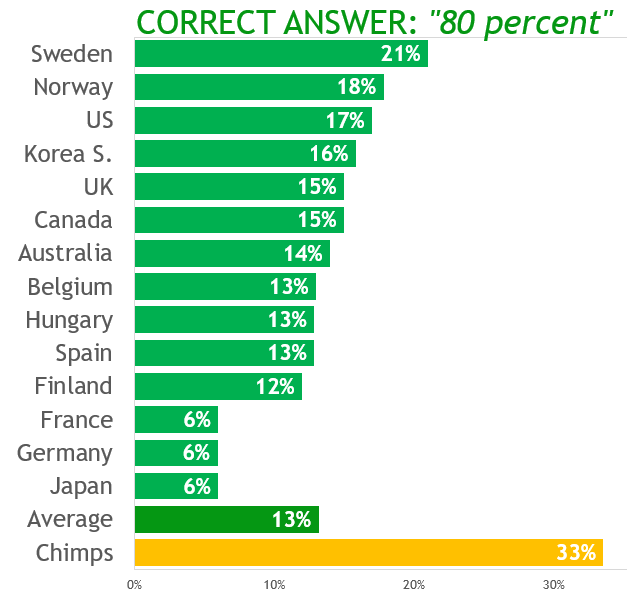
\includegraphics[scale=0.35]{img/vax_q.png}
\end{center}
\end{frame}

\begin{frame}{School}
\begin{center}
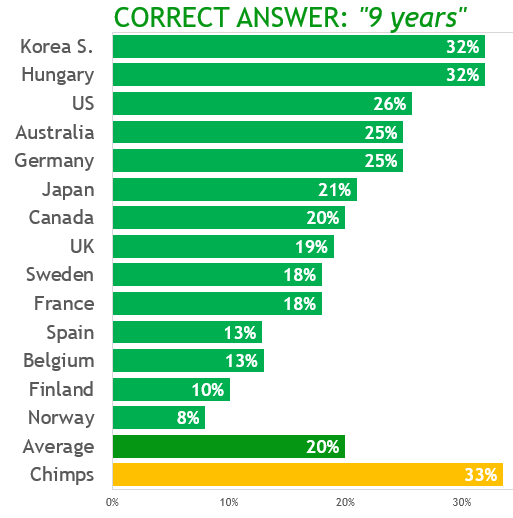
\includegraphics[scale=0.4]{img/school_q.png}
\end{center}
\end{frame}

\begin{frame}{Dots}
Which of these boxes look random?
\begin{center}
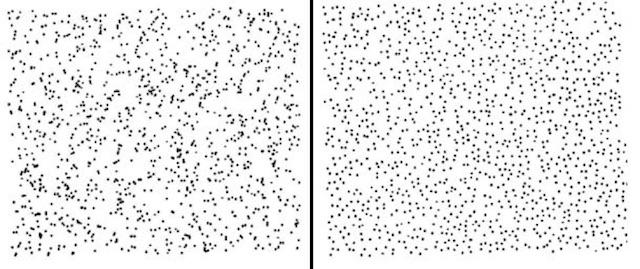
\includegraphics[scale=0.4]{img/random_dots.jpg}
\end{center}
\end{frame}

\begin{frame}{Why do we need statistics?}

Human beings are great at identifying patterns
\begin{itemize}
\item Cognitive biases
\item Poor intuition of uncertainty and randomness
\end{itemize}
\vspace{4mm}

\textbf{Statistics} gives us a framework for answering questions about the world using data (scientific method)

\begin{enumerate}
\item Construct a hypothesis
\item Collect data
\item Consider evidence
\item Draw conclusions
\end{enumerate}

\end{frame}

\begin{frame}{Populations and Parameters}
A \textbf{population} is a constrained group of subjects/events/things about which we wish to ask a scientific question \vspace{4mm}

A \textbf{parameter} is a \textit{quantifiable} attribute of a population. It is often assumed to be a fixed value within the bounds of the population \vspace{4mm}

A \textbf{census} is a complete collection of data for a population. This lets us exactly determine the value of a parameter within the population

\end{frame}

\begin{frame}{Samples and Statistics}

A \textbf{sample} is (often) a much smaller, (generally) \textit{randomly collected} subgroup of a larger population \vspace{4mm}

A \textbf{statistic} is an \textit{estimate} of a parameter that we get using data collected from the sample

\end{frame}



\begin{frame}{The Statistical Framework}
\begin{center}
\usetikzlibrary{decorations.pathreplacing,positioning, arrows, shapes, calc,shapes.multipart}
\tikzstyle{block1} = [rectangle, draw, fill=yellow!20, 
    text width=10em, text centered, rounded corners, minimum height=6em]
\tikzstyle{block2} = [rectangle, draw, fill=yellow!20, 
    text width=5em, text centered, rounded corners, minimum height=3em]
\tikzset{
    %Define standard arrow tip
    >=stealth,
    % Define arrow style
    pil/.style={
           ->,
           thick,
           shorten <=2pt,
           shorten >=2pt,}
}
\tikzstyle{line} = [draw, -latex]
\begin{tikzpicture}[node distance = 3cm, auto]
            % Place nodes
            \node [block1] (pop) {Population \\ (Parameter)};
            \node [block2, below of=pop] (samp) {Sample \\ (Statistic)};
            
            % Draw edges
            \draw[<-, >=latex, shorten >=2pt, shorten <=2pt, bend right=45, thick]  (pop.west) to node[auto, swap] {Inference}(samp.west);
            \draw[<-, >=latex, shorten >=2pt, shorten <=2pt, bend right=45, thick] (samp.east) to node[auto, swap] {Study Design}(pop.east); 
            
        \end{tikzpicture}
  \end{center}
\end{frame}

\begin{frame}{Population and Samples}
\begin{center}
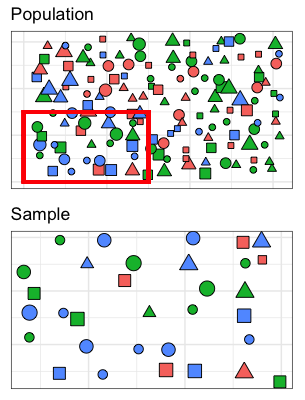
\includegraphics[scale=0.5]{img/pop_sample.png}
\end{center}
\end{frame}

\begin{frame}{An example}
Suppose we are interested in determining the average height of students currently enrolled at Grinnell College  \vspace{4mm}

Does it matter \textit{which} students we sample? \vspace{4mm}

Does it matter \textit{how many} students we sample? \vspace{4mm}

\end{frame}
%
%\begin{frame}{Sample Variability and Error}
%It is unlikely that the \textit{statistic} derived from our sample matches the \textit{parameter} of our population exactly
%
%\begin{itemize}
%
%\end{itemize}
%
%\end{frame}
%
%\begin{frame}{Some considerations}
%The goal is to draw conclusions from a broader population based on what we observe in a sample. As such, it is important that our sample is \textbf{representative} of our population \vspace{3mm}
%
%\textbf{Bias} describes the phenomenon in which the characteristics of our sample deviate from those of the population in important ways
%\begin{itemize}
%\item Non-response bias
%\item Convenience bias
%\item Confounding bias
%\end{itemize}
%\end{frame}

%\begin{frame}{An example}
%Suppose we are interested in determining the average height of students currently enrolled at Grinnell College  \vspace{8mm}

%It is unlikely that the \textit{statistic} (average height) derived from our sample matches the \textit{parameter} (average height) of our population exactly
%\end{frame}


\begin{frame}{Some definitions}

An \textbf{observation} (sometimes called an observational unit or case) is the subject/thing we are collecting data from \vspace{4mm}

Characteristics of an observation are known as \textbf{variables}. Variables typically come in one of two types: \vspace{4mm}

\begin{enumerate}
\item \textbf{Quantitative Variable:} Typically data that is stored in the form of \textit{numbers}, and is numerical in nature
\begin{itemize}
\item Continuous data i.e., height and weight
\item Discrete data (only specific values allowed) i.e., points scored in a game
\end{itemize} \vspace{2mm}
\item \textbf{Categorical Variable:} variables that are naturally divided into \textit{groups} \vspace{-2mm}
\begin{itemize}
\item Binary (two groups)
\item Nominal (no ordering) ex: eye color
\item Ordinal (ordering makes sense) ex: year in college (F/J/So/Se)
\end{itemize}
\end{enumerate}
\end{frame}

\begin{frame}{Variables}
\begin{center}
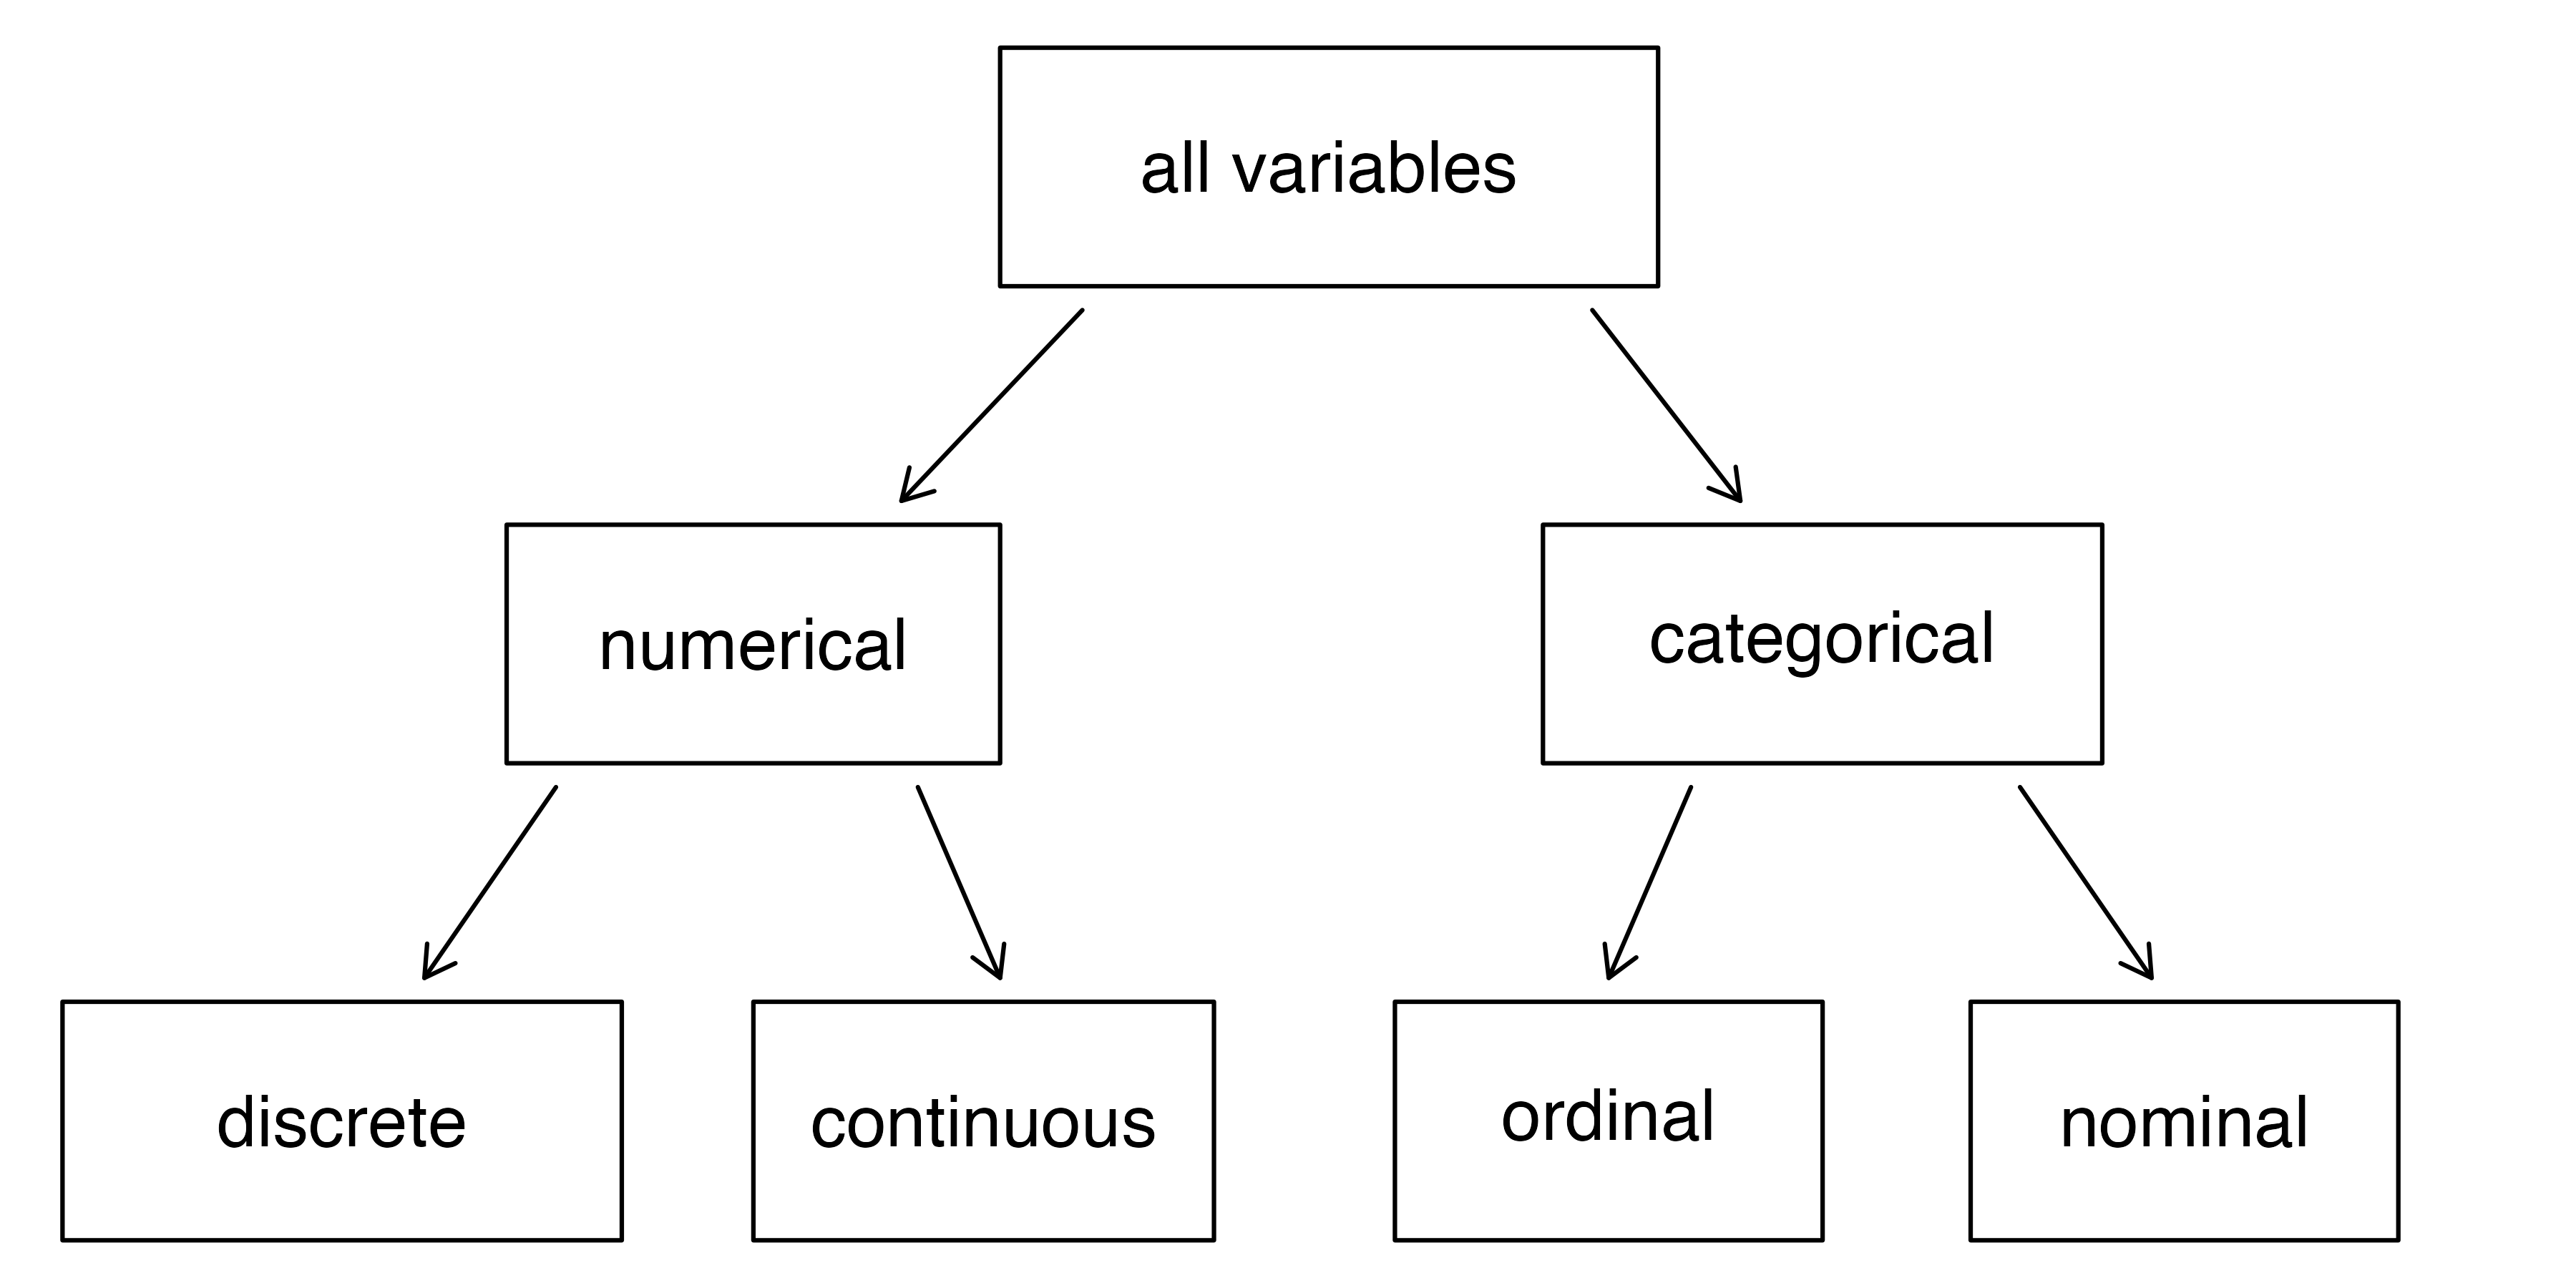
\includegraphics[scale=0.6]{img/data_vars.png}
\end{center}
\end{frame}

\begin{frame}{Gray areas}

The type of variable dictates how we analyze it:
\begin{itemize}
\item We often use the \textbf{mean} or \textbf{average} to analyze quantitative variables
\item We often use \textbf{proportions} or \textbf{percentages} to analyze categorical variables
\end{itemize}

\vspace{4mm}

Sometimes there are situations in which a variable is technically one type, but it may be more useful to analyze it as another. Sometimes the type of variable can be different depending on how we record or organize our data. 

\end{frame}

\begin{frame}{Gray areas}
Take a few minutes to discuss these questions with those around you, whether these might be used as quantitative or categorical variables:

\begin{enumerate}
\item Grades for a statistics class
\item A Likert Scale with five levels, measuring pain from "None at all" to "Extreme"
\item The year of birth for people enrolled in STA-209
\end{enumerate}

\vspace{4mm}
\textit{``An approximate answer to the right problem is worth a good deal more than an exact answer to an approximate problem." \\ John Tukey, Statistician}

\end{frame}

\begin{frame}{Key Takeaways}

\begin{itemize}
\item Statistics, as a discipline, gives us tools for analyzing variability in our data and answering scientific questions
\item Parameters are quantifiable attributes of populations that we are interested in study. A sample is a subset of a population, and a statistic is an estimate of a parameter that we calculate using data from the sample
\item An observation is the smallest unit of study within a population. It's charactersistics are called variables
\item Variables primarily come in two types:
\begin{itemize}
\item Quantitative
\begin{itemize}
\item Continuous (height)
\item Discrete (number of people)
\end{itemize}
\item Categorical
\begin{itemize}
\item Binary (disease status)
\item Nominal (favorite color)
\item Ordinal (educational attainment)
\end{itemize}
\end{itemize}
\end{itemize}

\end{frame}

\begin{frame}{Knowledge Check}
Why do we need statistics? \vspace{3mm}

How would you describe the statistical framework to a relative? \vspace{3mm}

What is an observation and how do we describe its characteristics? \vspace{3mm}

What types of variables are there, and when is each appropriate?
\end{frame}

\begin{frame}{Summary}
Statistics is a domain agnostic tool that allows us to make quantitative statements about a population \vspace{3mm}

Most data that we encounter will be categorical or quantitative in nature \vspace{4mm}

\textbf{Next Time:}
\begin{itemize}
\item Introduction to R
\item Read Sections 1.2.1, 1.2.2, and 1.2.3 from IMS
\end{itemize}
\end{frame}


%
%\begin{frame}{Summarizing Data}
%Here, for example, are 20 observations out of 244 regarding the tips given to one waiter over the course of several months in one restaurant:
%
%\begin{table}[ht]
%\tiny
%\centering
%\begin{tabular}{rrllllr}
%  \hline
%Total Bill & Tip & Sex & Smoker & Day & Time & Size \\ 
%  \hline
%13.42 & 1.58 & Male & Yes & Fri & Lunch &   2 \\ 
%  16.27 & 2.50 & Female & Yes & Fri & Lunch &   2 \\ 
%  10.09 & 2.00 & Female & Yes & Fri & Lunch &   2 \\ 
%  20.45 & 3.00 & Male & No & Sat & Dinner &   4 \\ 
%  13.28 & 2.72 & Male & No & Sat & Dinner &   2 \\ 
%  22.12 & 2.88 & Female & Yes & Sat & Dinner &   2 \\ 
%  24.01 & 2.00 & Male & Yes & Sat & Dinner &   4 \\ 
%  15.69 & 3.00 & Male & Yes & Sat & Dinner &   3 \\ 
%  11.61 & 3.39 & Male & No & Sat & Dinner &   2 \\ 
%  10.77 & 1.47 & Male & No & Sat & Dinner &   2 \\ 
%  15.53 & 3.00 & Male & Yes & Sat & Dinner &   2 \\ 
%  10.07 & 1.25 & Male & No & Sat & Dinner &   2 \\ 
%  12.60 & 1.00 & Male & Yes & Sat & Dinner &   2 \\ 
%  32.83 & 1.17 & Male & Yes & Sat & Dinner &   2 \\ 
%  35.83 & 4.67 & Female & No & Sat & Dinner &   3 \\ 
%  29.03 & 5.92 & Male & No & Sat & Dinner &   3 \\ 
%  27.18 & 2.00 & Female & Yes & Sat & Dinner &   2 \\ 
%  22.67 & 2.00 & Male & Yes & Sat & Dinner &   2 \\ 
%  17.82 & 1.75 & Male & No & Sat & Dinner &   2 \\ 
%  18.78 & 3.00 & Female & No & Thur & Dinner &   2 \\ 
%   \hline
%\end{tabular}
%\end{table}
%
%\end{frame}
%
%\begin{frame}{Univariate Data -- Categorical}
%A \textit{barchart} is often used to tally the frequencies of a categorical variable
%\begin{center}
%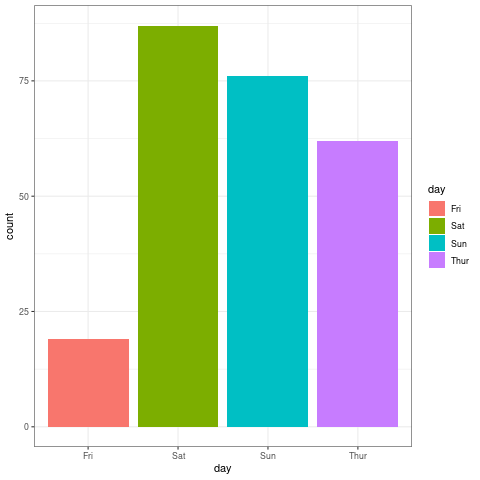
\includegraphics[scale=0.35]{img/tip_day.png}
%\end{center}
%\end{frame}
%
%\begin{frame}{Univariate -- Quantitative}
%For quantitative variables, a \textit{histogram} is often used to show the distribution of values
%\begin{center}
%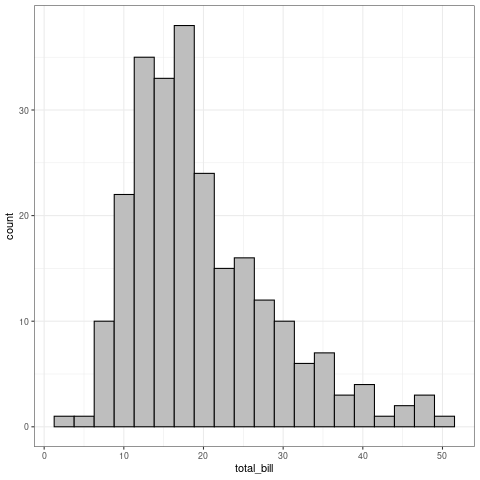
\includegraphics[scale=0.35]{img/bill_bin_20.png}
%\end{center}
%\end{frame}
%
%\begin{frame}{Univariate -- Quantitative}
%\begin{columns}
%
%  \begin{column}{0.45\textwidth}
%	\begin{center}
%	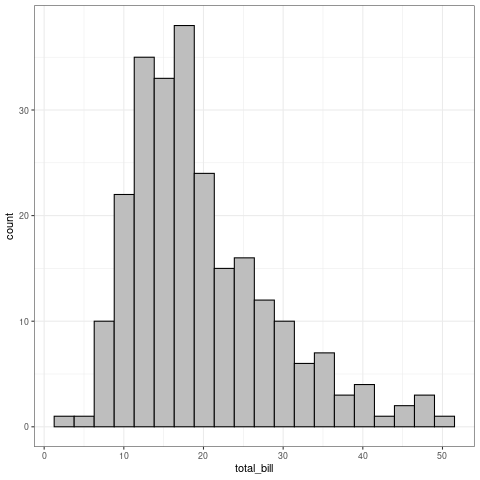
\includegraphics[scale=0.35]{img/bill_bin_20.png}
%	\end{center}
%  \end{column}
%  \begin{column}{0.45\textwidth}
%	Here, there is quite a bit more we can examine:
%	\begin{itemize}
%	\item Where does the ``center" appear to be?
%	\item How spread out is this data?
%	\item What about the range of this data?
%	\item Does it appear skewed?
%	\end{itemize}
%  \end{column}
%
%\end{columns}
%\end{frame}
%
%\begin{frame}{Univariate -- Quantitative}
%\begin{center}
%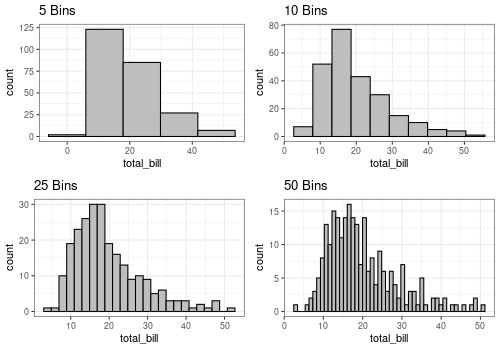
\includegraphics[scale=0.5]{img/bin_grid.png}
%\end{center}
%\end{frame}
%
%\begin{frame}{Bivariate Visual Summaries}
%Often, a statistical analyses is motivated by an investigator looking for a relationship between two or more variables \vspace{2mm}
%
%When there does appear to be some connection between two variables, we say that they are \textbf{associated}. Variables that are \textit{not} associated are said to be \textit{independent} \vspace{2mm}
%
%We typically identify one variable as being the \textbf{response} or \textbf{dependent variable}, with the remaining variables being \textbf{explanatory} or \textbf{independent variable} 
%
%\begin{align*}
%\text{explanatory variable} \rightarrow might \ affect \rightarrow \text{response variable}
%\end{align*}
%
%This is meant in a \textit{predictive} context, rather than a necessarily \textit{causal} one
%
%\end{frame}
%
%\begin{frame}{Bivariate -- Stacked Bar}
%The first type of bivariate bar chart is known as a \textbf{stacked bar chart}, which allows us to break down one variable in terms of another. Here, we consider if any smokers were included in the party
%
%\begin{center}
%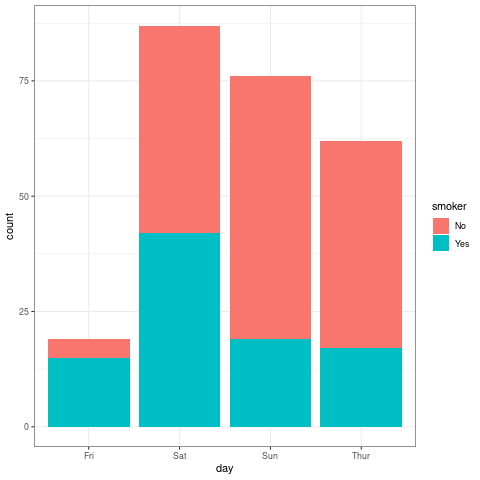
\includegraphics[scale=0.35]{img/bar_stacked.png}
%\end{center}
%
%\end{frame}
%
%\begin{frame}{Bivariate -- Dodge Bar}
%The second type of bivariate bar chart is known as a \textbf{dodged bar chart}, which presents both variables alongside one another. This makes comparing within groups much simpler
%
%\begin{center}
%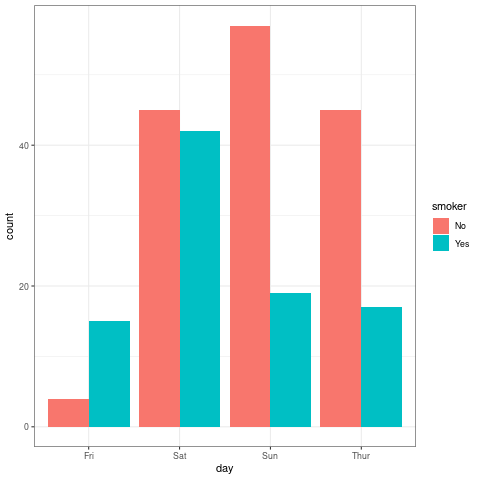
\includegraphics[scale=0.35]{img/bar_dodge.png}
%\end{center}
%
%\end{frame}
%
%\begin{frame}{Bivariate -- Filled Bar}
%The last type of bivariate bar chart is known as a \textbf{filled bar chart}, offering proportions. Although we lose absolute counts, we can now see relative frequencies within each group
%
%\begin{center}
%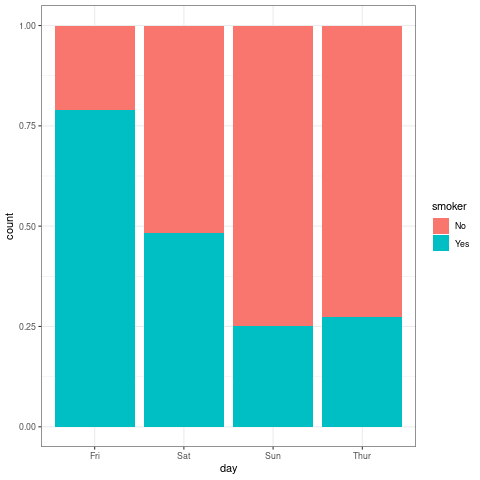
\includegraphics[scale=0.35]{img/bar_fill.png}
%\end{center}
%
%\end{frame}
%
%\begin{frame}{Bar chart quesiton}
%fill
%\end{frame}
%
%\begin{frame}{Scatterplots}
%Visual summaries investigating the relationship between two quantitative variables are often presented with a \textbf{scatterplot} \vspace{2mm}
%\begin{columns}
%
%  \begin{column}{0.5\textwidth}
%  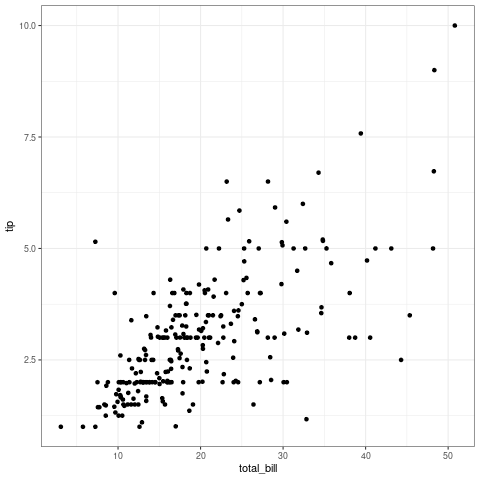
\includegraphics[scale=0.35]{img/scatter_tip.png}
%  \end{column}
%  \begin{column}{0.4\textwidth}
%  What kind of relationship do we see between the total bill and the tip amount?
%  \end{column}
%
%\end{columns}
%\end{frame}
%
%\begin{frame}{Types of Quantitative Relationships}
%\begin{center}
%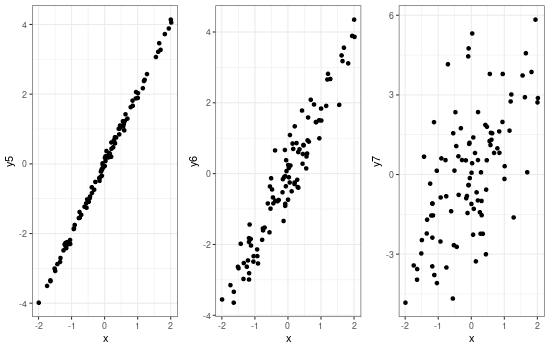
\includegraphics[scale=0.5]{img/linear_strong.png}
%\end{center}
%\end{frame}
%
%
%\begin{frame}{Types of Quantitative Relationships}
%\begin{center}
%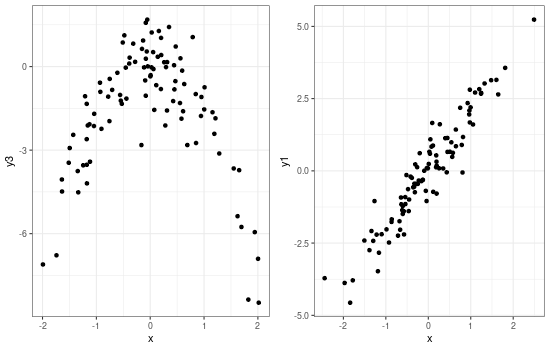
\includegraphics[scale=0.5]{img/linear_nonlinear.png}
%\end{center}
%\end{frame}
%
%\begin{frame}{Types of Quantitative Relationships}
%\begin{center}
%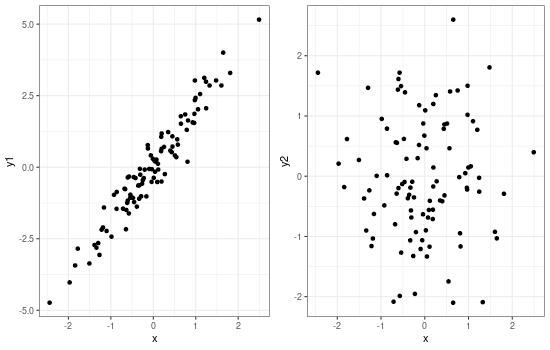
\includegraphics[scale=0.5]{img/linear_none.png}
%\end{center}
%\end{frame}
%
%
%\begin{frame}{Summary}
%blah blah blah \\
%
%homework + reading
%\end{frame}

\begin{frame}{Sources}
IMS textbook \\
Professor Miller's and Professor Nolte's course notes\\
Dr. Ziegler's (ISU) course notes

\end{frame}





%\begin{frame}
%\begin{columns}
%
%  \begin{column}{0.45\textwidth}
%%
%  \end{column}
%  \begin{column}{0.45\textwidth}
%%
%  \end{column}
%
%\end{columns}
%\end{frame}



%%%%%%%%%%%%%%%%


\end{document}
